\chapter{二次量子化}
今天是2019年7月13日,暑假正式开始.在学习统计物理学中的第十二章 {\bf \S 117 简并气体中的密度涨落关联 }时用到了量子力学中的二次量子化方法,但是作为考研的准备,对于二次量子化并没有太多的研究,同时理解起来有一定的难度,但是作为学习之用我感觉到了二次量子化的重要性,所以集中几天的时间学习理解二次量子化.学习的基础是朗道《量子力学(非相对论)》,由于长时间没有集中精力学习量子力学所以导致最近几天十分头疼,理解之后记录这一章的核心内容.\footnote{这一章对应量子力学{\bf 第九章 粒子的全同性}}

\section{同类粒子的不可分辨原理}

微观领域物体的运动是遵守量子力学规律的.比如两个电子,如果它们服从经典力学,则我们可以分辨它们.方法是记录它们开始运动的位置,然后按按照刘维定理,每个粒子都有确定的轨道,所以分辨出轨道就分辨出电子了.但是实际情况不是这样,比如在某一时刻,我们确定的电子的位置,但是在任意小的任意时刻我们不能给出电子的确切位置,所以根本无法按照经典力学定义速度!因为经典速度指当$\Delta t$ 趋近零时,位移与时间的比值,但是这里既然位移无法给出,则速度也就无从谈起,所以也不会有轨道了.因此在量子力学的意义上,我们即使开始给粒子编了号,但是在任意小的一段时间内,我们无法说明到底是检测到了哪一个粒子.在量子力学的层面上我们谈论的问题就变成了在哪个位置发现了几个电子,且能够发现几个电子的概率是多少.


由于同类粒子的不可分辨原理,我们在描述粒子的时候只能写出这些粒子所满足的量子力学方程,并确定它们所遵守的波函数.但是根据Schr\"odinger 方程所确定的波函数,还有一个不会影响相对概率分布的相角,这一点需要注意.由于粒子不可分辨,所以在交换粒子时波函数将会发生一些变化,交换粒子意味着对换波函数中两个粒子的所有坐标.而粒子又是不可分辩的,所以交换任意两个全同粒子的坐标后,波函数的变化是不会导致相对概率的变化的,也就是最多出现一个相因子,即
\begin{gather}
  \Psi(\xi_1,\xi_2)=e^{i\alpha}\Psi(\xi_2,\xi_1)
  \intertext{再对换一次粒子,则波函数必然变回原来的样子,即}
  \Psi(\xi_1,\xi_2)=e^{i2\alpha}\Psi(\xi_1,\xi_2)
  \intertext{基于波函数的任意性,所以必然有}
  e^{i2\alpha}=1
  \intertext{解得}
  e^{i\alpha}=\pm 1
  \intertext{所以对于波函数就有两种情况}
  \Psi(\xi_1,\xi_2)=\pm\Psi(\xi_2,\xi_1)
\end{gather}
对于交换粒子后波函数取正的情况,我们称满足这个情况的粒子为Bose 子,对于交换粒子后波函数改变一个负号的情况,我们称满足这个情况的粒子为Fermi 子.

根据不同类型的粒子我们可以先从Schr\"odinger 方程解出任意一个解,然后再构造出满足交换规律的波函数.首先,我们从某一个满足Schr\"odinger 方程的函数出发,构造满足对称性的N个Bose 子的波函数形式.记量子态分别为$p_1,p_2,\cdots $ ,同时各粒子用不同的坐标$\xi_1,\xi_2,\cdots $ 来表示,如果两个粒子处于相同的状态,则$p$值相同,但是它们的坐标仍然是已经标定的标号.所以要满足每一对粒子交换都是对称的,则可以如下构造
\begin{gather}
  \Psi = \Sigma \Psi_{p_1}(\xi_1)\Psi_{p_2}(\xi_2)\cdots\Psi_{p_N}(\xi_N) 
\end{gather}
上式中$\Sigma$ 表示对于所有可能的交换求和,在上式中可以理解各$p_i$不动,交换各个坐标$\xi_i$,也可以理解为各 $\xi_i$ 不动,改变各$p_i$,其数学结果是一样的,可以验证我们对于$\Psi$ 而言交换任意两个粒子,其波函数都是对称的.

在上式中所构造的波函数并没有归一化.因为有可能粒子处于同一个状态,比如有$N_1$个粒子处于$\Psi_{p_1}$态,这是有可能的.因为对于处于同一状态的粒子的交换不能产生新的态,所以在各种交换中会出现相同的态,那么各种求和的可能性中总共有项数
\begin{gather}
  \frac{N!}{N_1!N_2!\cdots N_m!} 
\end{gather}
所以得归一化的波函数为
\begin{gather}
  \Psi =\sqrt{\frac{N_1!N_2!\cdots N_m!}{N!}} \Sigma \Psi_{p_1}(\xi_1)\Psi_{p_2}(\xi_2)\cdots\Psi_{p_N}(\xi_N) 
\end{gather}
此时上面的求和应当理解为对所有粒子交换再求和,因为相同的态下粒子的交换,已经由$N_i!$ 而除去了.在上面的下标中,应当理解为$p_1=p_2=\cdots =p_{N_1}$,$p_{N_1}=p_{N_1+1}=\cdots =p_{N_1+N_2}$ ,$\cdots \cdots$.

对于Fermi 子,我们可以构造成如下波函数
\begin{equation}
  \Psi=\frac{1}{\sqrt{N!}}
  \begin{vmatrix}
    \Psi_{p_1}(\xi_1)&\Psi_{p_1}(\xi_2)&\cdots&\Psi_{p_1}(\xi_N)\\
    \Psi_{p_2}(\xi_1)&\Psi_{p_2}(\xi_2)&\cdots&\Psi_{p_2}(\xi_N)\\
    &&\vdots &\\
    \Psi_{p_N}(\xi_1)&\Psi_{p_N}(\xi_2)&\cdots&\Psi_{p_N}(\xi_N)
  \end{vmatrix}
\end{equation}
很显然,在式中交换任意两列或者两行,则波函数都会改变一个负号.同时,不可能有两行是相同的,即$p_i\neq p_j, i\neq j$,如果有两行相同,则行列式为零,此即 泡利不相容原理---同一时刻不可能有两个相同的费米子处于相同的态.

\section{交换作用}

在没有磁场的情况下解Schr\"odinger 方程,我们会得到一系列的解和能级.由于在这种情况下能级中不含自旋,所以导致它不能完全反映波函数的对称性.也就是说,波函数的对称性会对这些解中的一些波函数给出限制,有一些在某种情况下将是不允许的.在这种情况下,波函数可以写成坐标函数和自旋函数的乘积,即
\begin{equation}
  \Psi(\xi_1,\xi_2,\cdots,\xi_n)=\varphi(r_1,r_2,\cdots ,r_N)\cdot X(\sigma_1,\sigma_2,\cdots ,\sigma_n)
\end{equation}
当考虑的是玻色子的时候,要求$\Psi(\xi_1,\xi_2,\cdots ,\xi_N)$为对称波函数,所求的坐标波函数$\varphi(r_1,r_2,\cdots,r_N)$ 如果为对称的,则自旋波函数$X(\sigma_1,\sigma_2,\cdots ,\sigma_n)$ 也是对称的,反之都是反对称的.当所考虑的是费米子时,要求$\Psi(\xi_1,\xi_2,\cdots ,\xi_N)$为反对称波函数,如果坐标波函数$\varphi(r_1,r_2,\cdots,r_N)$ 如果为对称的,则自旋波函数$X(\sigma_1,\sigma_2,\cdots ,\sigma_n)$ 是反对称的,反之则坐标波函反对称,自旋波函对称.但是如果不去考虑这个对称性,则仅有坐标部分求得的波函数和能级就要比考虑了对称性时要多,于是考虑交换对称性会影响到实际的波函和能级.

多电子系统的那些能量允许的值依懒于该系统的总自旋.由于这个原因,我们可以把这种依懒关系说成是粒子间的一种特殊作用的结果.这种作用称为``{\bf 交换作用}''.\footnote{引用自《量子力学(非相对论)》第213页.}

一个自旋为$s$ 的粒子A,它在$z$ 轴方向的投影有$2s+1$个.如果考虑一个复合粒子B,它由$2s$个自旋为$\frac{1}{2}$ 的基本粒子构成,由角动量的合成规则可得,这个复合粒子的最大角动量为$s$,从物理上讲,一个自旋为$s$粒子和这里所述的复合粒子是等价的,从描述方法上来说,不会有什么不同.对于这个复合粒子,它可以由一个$2s$秩旋量来描述,即
\begin{equation}
  X^{\overbrace{\alpha\beta\cdots}^{\text{共2s项}}}
\end{equation}
当粒子A在$z$轴上的分量为$\sigma$ 时,此分量对应如下B的分量
\begin{equation}
  X^{\overbrace{11\cdots}^{s +\sigma}\overbrace{22\cdots}^{s -\sigma}}
\end{equation}
显然B的旋量所表示的自旋在$z$轴上的分量值为$\frac{1}{2}(s+\sigma)-\frac{1}{2}(s-\sigma)=\sigma$,所以分量上来讲也是对应的.复合粒子由$2s$个自旋为$\frac{1}{2}$的全同粒子构成,所以在上述表达式上,哪些粒子取$1$,哪些粒子取$2$,这是不确定的.这就产生以确定具体对应关系的问题,记A的此分量为$\Psi(\sigma)$,则考虑下式成立
\begin{equation}
  \sum_{\sigma=-s}^{s} |\Psi(\sigma)|^2 =\sum_{\alpha\beta\cdots =1}^2 |X^{\alpha\beta\cdots}|^2
\end{equation}
上式确定了在空间一点粒子出现的概率,因为它考虑到了各个自旋的概率出现的和.显然,右式中出现$\sigma$ 的项共有$\frac{(2s)!}{(s+\sigma)!(s-\sigma)!}$ 项,同时又考虑到$s$的任意性,所以可以确定具体对应系为
\begin{equation}
  \Psi(\sigma)=
  \sqrt{\frac{(2s)!}{(s+\sigma)!(s-\sigma)!}}
    X^{\overbrace{11\cdots}^{s+\sigma}\overbrace{22\cdots}^{s-\sigma}}
\end{equation}
需要说明的是在上式中旋量,我们取出了一个任意的分量,将其中所有$1$并到一块,所有的$2$ 并到了一块,当$\sigma$ 增加$1$ 时,在$1$这一分组追加一个,同时在$2$分组减少一个就好.同时在计算项数的数目时,当$s$主半整数时,$s\pm \sigma$也是整数,所以在讨论问题的过程中是兼顾了半整数的.

下面考虑第213页的所述的双粒子系统,每个粒子的自旋为$s$,则需要一个$4s$秩的旋量来描述.即
\begin{equation}
  X^{\overbrace{\nu\mu\cdots}^{2s}\overbrace{\rho\sigma\cdots}^{2s}}
\end{equation}
这两个粒子所能构成的系统的总自旋为$0$,$1$,$2$,$\cdots$,$2s$,当总自旋为$S$,相当于将上述自旋缩并掉$2s-S$个指标,而变成一个$2S$秩旋量,其自旋就是$S$.缩并意味着,可以通过将后$2s-S$个指标移到下标上来,按Einstein 约定,哑标求和.即
\begin{equation}
  X^{\overbrace{\nu\mu\cdots}^{S}\overbrace{\rho\sigma\cdots}^{S}
  \overbrace{\rho'\sigma'\cdots}^{2s-S}}\ _{\underbrace{\rho'\sigma'\cdots}_{2s-S}}
\end{equation}
当交换所有粒子时相当于交换$\nu$,$\mu$,$\cdots$,$\nu'$,$\mu'$,$\cdots$ 和$\rho$,$\sigma$,$\cdots$,$\rho'$,$\sigma'$,$\cdots$ 两组指标.当交换上标和下标时,旋量会改变符号,所以交换粒子后,此复合粒子的旋量改变为$(-)^{2s-S}$.

同时考虑整体的波函,当交换两个粒子时,则完整波函数符号改变为$(-)^{2s}$,所以可得坐标波函的符号改变为 $(-)^S$.这样的我们就可以得到结论:\CJKunderwave{由两个全同粒子所构成的系统,当总自旋为偶数时,坐标波函为对称的,当总自旋为奇时,坐标波函为反对称的.}

下面讨论一下该系统中具有偶数或奇数$S$值的不同状态各有多少个.这个问题我可以给出我的一个讨论方式.每个自旋为$s$的粒子,由于在$z$轴上分量可以有$2s+1$个,所以总的状态数为$(2s+1)^2$个.当$s$为整数时,对于偶数$S$,则可以分为两类构成,如果两个粒子的$z$轴分量相同,则一共有$2s+1$个,另一部分由两个粒子不同的分量构成,它一共有$2s(2s+1)$种,这些不同的分量所构成的自旋奇偶各半,所以由其所构成的偶数$S$值共有$s(2s+1)$,因此总共有偶数的$S$值的数目为$(s+1)(2s+1)$,有奇数的 $S$值数目为$s(2s+1)$.同理,当$s$为半整数时,$2s+1$个相同的$z$分量,构成的是奇数$S$,所以奇数$S$值共有$(s+1)(2s+1)$个,此时偶数$S$值有$s(2s+1)$个.

下面再按朗道的方式讨论一下:两个粒子,每个粒子自旋为 $s$ ,所以总自旋的 $S$ 数值可以为$0$ ,$1$ ,$2$ ,$3$ ,$\cdots$,$2s$ ,对于每一个$S$ 值可以有$2S+1$个分量,所以当$s$为整数时,$S$为偶数的情况为
\begin{align}
  \sum_{S=0,2,4,\cdots, 2s}(2S+1)
  &=4\sum_{k=1,2,\cdots , s} k + (s+1)\notag\\
  &=4\cdot \frac{s(s+1)}{2}+(s+1)\notag\\
  &=(s+1)(2s+1)
\end{align}
所以$S$为奇的情况为
\begin{equation}
  (2s+1)^2-(s+1)(2s+1)=s(2s+1)
\end{equation}
同理,当$s$为半整数时,可以得到偶数$S$值的态数共有$s(2s+1)$,奇数$S$值态数有$(s+1)(2s+1)$个.对比两个方法,我觉得朗道的方法直接求解来的更直接,我考虑的方法可以更快的写出答案,各有长短.

\section{置换对称性}

这一节的讨论由于我是首次接触,所以消耗了较长时间来理解杨图的,对于全同粒子,它的完整波函数是对称的或者是反对称的.在非相对论范围,可以通过求解Schr\"odinger 方程来得到坐标函数,但是整体波函数是坐标函数和自旋波函数的乘积.整体的对称性或反对称性是必然的,但对于坐标的波函数不一定总是能实现反对称性,至于对称性是可以通过对称化手续来解决的,所以具体的情况就变的很复杂.同时,由多个粒子构成的系统,同一个坐标函数所描述的态上可能有多个粒子,这些粒子的交换不能带来新的态.假设$N$个粒子所包含的坐标函数一共有$m$个,而粒子数为$N$,我们面临的问题是将这$N$个粒子分配到这$m$态中,第$i$ 态中所具有粒子数为$N_i$个,所以有
\begin{gather}
  N=N_1+N_2+\cdots +N_m
\end{gather}
其中第$i$ 态的波函数我们总是可心通过对称化手续使其对称化,但是不能反对称化,因为反对称化相同态结果为零.所以反对称化只能出现在\CJKunderwave{不同量子态之间}.第$i$ 态波函数记为
\begin{gather}
  \varphi_i(r_1,r_2,\cdots,r_{N_i})
\end{gather}
我们考虑将5 个粒子分配两个不同的态中,其中第一个态有3个粒子,第二个态中有2个粒子,这两个态认为已经对称化的.则波函数我们首先取为
\begin{gather}
  \Psi^{(0)}=\varphi_1(r_1,r_2,r_3)\varphi_2(r_4,r_5) 
\end{gather}
上述波函数,满足$r_1,r_2,r_3$之间相互交换是对称的,$r_4,r_5$之间交换是对称的.我们再考虑将其反对称化,看看能处理到什么程序.由于粒子是全同的,而不同态之间才可以反对称化,所以可以任选$r_1$和$r_4$,使其反对称化,则得到
\begin{gather}
  \Psi^{(1)}=\frac{1}{\sqrt{2}}
  \{
    \varphi_1(r_1,r_2,r_3)\varphi_2(r_4,r_5) 
    -\varphi_1(r_4,r_2,r_3)\varphi_2(r_1,r_5) 
  \}
\end{gather}
我们看到在将函数$\Psi^{(0)}$变换为$\Psi^{(1)}$ 时粒子的分配关系仍然是$3,2$分配的,它没有变,又因为是全同粒子,所以在物理上也没有什么不同.但是仔细观察这两个函数,$\Psi^{(1)}$ 关于$r_1$ 和$r_4$是反对称的,但是由于$r_2,r_3$并没有参与变换,所以显然它对$r_2,r_3$仍然保持对称的.但是$r_1,r_2$将不再保持对称!即 
\begin{gather}
  \frac{1}{\sqrt{2}}
  \{
    \varphi_1(r_1,r_2,r_3)\varphi_2(r_4,r_5) 
    -\varphi_1(r_4,r_2,r_3)\varphi_2(r_1,r_5) 
  \}
  \neq
  \frac{1}{\sqrt{2}}
  \{
    \varphi_1(r_2,r_1,r_3)\varphi_2(r_4,r_5) 
    -\varphi_1(r_4,r_1,r_3)\varphi_2(r_2,r_5) 
  \}\notag
\end{gather}
上式表明,一般对两个粒子做了反对称变换,则原来它们各自的对称状态将会被破坏!我们可以用上述方法讨论下去,但是一直这样变换下去,书写将变的混乱,所以杨图的作用也就在这里.我们将粒子的分组,按数目排成行,然后再按由多到少的顺序排列下来,例如上述的$5=3+2$分割,可以表达为
\begin{figure}[H]
  \centering
  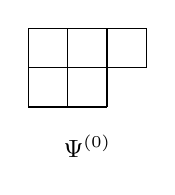
\begin{tikzpicture}
    \draw (0,0)--(1.5,0);
    \draw (0,-0.5)--(1.5,-0.5);
    \draw (0,-1)--(1,-1);
    \foreach \x in {0,0.5,1,1.5} 
    \draw (\x,0)--(\x,-0.5);
    \foreach \x in {0,0.5,1} 
    \draw (\x,-0.5)--(\x,-1);
    \draw (0.75,-1.5) node {\small $\Psi^{(0)}$};
  \end{tikzpicture}
  \quad
  \begin{tikzpicture}
    \draw (0,0)--(1.5,0);
    \draw (0,-0.5)--(1.5,-0.5);
    \draw (0,-1)--(1,-1);
    \foreach \x in {0,0.5,1,1.5} 
    \draw (\x,0)--(\x,-0.5);
    \foreach \x in {0,0.5,1} 
    \draw (\x,-0.5)--(\x,-1);
    \draw[pattern=north west lines] (0,0) rectangle (0.5,-1);
    \draw (0.75,-1.5) node {\small $\Psi^{(1)}$};
  \end{tikzpicture}
  \quad
  \begin{tikzpicture}
    \draw (0,0)--(1.5,0);
    \draw (0,-0.5)--(1.5,-0.5);
    \draw (0,-1)--(1,-1);
    \foreach \x in {0,0.5,1,1.5} 
    \draw (\x,0)--(\x,-0.5);
    \foreach \x in {0,0.5,1} 
    \draw (\x,-0.5)--(\x,-1);
    \draw[pattern=north west lines] (0,0) rectangle (1,-1);
    \draw (0.75,-1.5) node {\small $\Psi^{(2)}$};
  \end{tikzpicture}
  \caption{5=3+2}
  \label{fig:yangtu0}
\end{figure}
在图\ref{fig:yangtu0}中的第三个图$\Psi^{(2)}$,它表示在$\Psi^{(1)}$的基础上,再将$r_2$ 和$r_5$ 反对称化,所以$\Psi^{(2)}$ 也就是5个粒子按$3+2$ 分割时,所能达到的最大反对称程度.在以后的讨论中如果没有特殊声明,我们见到杨图\ref{fig:yangtu0}时应当按$\Psi^{(2)}$来理解,而不应当按变换中的状态$\Psi^{(0)},\Psi^{(1)}$理解,为了方便绘图,以后将不再绘出阴影.

下面按照$22=6+4+4+3+3+1+1$分割,我们来理解完整波函数区分成两部分乘积的时候,其构成对称和反对称的情形.

\begin{figure}[H]
  \centering
  \begin{tikzpicture}
    \draw (0,0)--(3,0); 
    \draw (0,-0.5)--(3,-0.5); 
    \foreach \x in {0,0.5,1,1.5,2,2.5,3}
    \draw (\x,0)--(\x,-0.5);
    \foreach \x in {0,0.5,1,1.5,2}
    \draw (\x,-0.5)--(\x,-1.5);
    \draw (0,-1)--(2,-1);
    \draw (0,-1.5)--(2,-1.5);
    \foreach \x in {0,0.5,1,1.5}
    \draw (\x,-1.5)--(\x,-2.5);
    \draw (0,-2)--(1.5,-2);
    \draw (0,-2.5)--(1.5,-2.5);
    \foreach \x in {0,0.5}
    \draw (\x,-2.5)--(\x,-3.5);
    \draw (0,-3)--(0.5,-3);
    \draw (0,-3.5)--(0.5,-3.5);
    \draw (1.5,-4) node {\small $A$};
    \draw[pattern=north west lines] (0,0) rectangle (0.5,-1);
  \end{tikzpicture}
  \quad
  \begin{tikzpicture}
    \draw (0,0)--(3,0); 
    \draw (0,-0.5)--(3,-0.5); 
    \foreach \x in {0,0.5,1,1.5,2,2.5,3}
    \draw (\x,0)--(\x,-0.5);
    \foreach \x in {0,0.5,1,1.5,2}
    \draw (\x,-0.5)--(\x,-1.5);
    \draw (0,-1)--(2,-1);
    \draw (0,-1.5)--(2,-1.5);
    \foreach \x in {0,0.5,1,1.5}
    \draw (\x,-1.5)--(\x,-2.5);
    \draw (0,-2)--(1.5,-2);
    \draw (0,-2.5)--(1.5,-2.5);
    \foreach \x in {0,0.5}
    \draw (\x,-2.5)--(\x,-3.5);
    \draw (0,-3)--(0.5,-3);
    \draw (0,-3.5)--(0.5,-3.5);
    \draw (1.5,-4) node {\small $B$};
    \draw[pattern=north west lines] (0,0) rectangle (0.5,-1);
  \end{tikzpicture}
  \caption{整体对称波函数}
  \label{fig:yangtu1}
\end{figure}

在图\ref{fig:yangtu1}中,两部分波函数的杨图完全相同,在每一行中所填充相同的粒子的不同变量(比如坐标函数用A表示,自旋函数用B表示).记A和B的乘积AB,即
\begin{gather}
  \Psi^{(1)}=\Psi_A\cdot \Psi_B
\end{gather}
交换第一行第一列和第二行第一列的粒子时,$\Psi_A$ 和$\Psi_B$ 都改变一个负号,所以乘积AB将不变号.但是根据杨图的构成规则,A和B的行不具有交换对称性,所以如果交换同一行中的两个粒子,则乘积AB不具备交换对称性.然而粒子的每一种交换,相当于N个粒子在两张杨图中的同步分配,当我们考虑到所有置换后的乘积,然后再叠加起来,这个叠加之后的波函数包含了各种可能的交换,当交换两个同行的粒子时,相当于改变了一下两个乘积的顺序,由于加法的交换律它不影响波函数.所以这个所有分配方式的和构成整体的波函数,即
\begin{gather}
  \Psi=\sum_i\Psi^{(i)}
\end{gather}

\begin{figure}[H]
  \centering
  \begin{tikzpicture}
    \draw (0,0)--(3,0); 
    \draw (0,-0.5)--(3,-0.5); 
    \foreach \x in {0,0.5,1,1.5,2,2.5,3}
    \draw (\x,0)--(\x,-0.5);
    \foreach \x in {0,0.5,1,1.5,2}
    \draw (\x,-0.5)--(\x,-1.5);
    \draw (0,-1)--(2,-1);
    \draw (0,-1.5)--(2,-1.5);
    \foreach \x in {0,0.5,1,1.5}
    \draw (\x,-1.5)--(\x,-2.5);
    \draw (0,-2)--(1.5,-2);
    \draw (0,-2.5)--(1.5,-2.5);
    \foreach \x in {0,0.5}
    \draw (\x,-2.5)--(\x,-3.5);
    \draw (0,-3)--(0.5,-3);
    \draw (0,-3.5)--(0.5,-3.5);
    \draw (1.5,-4) node {\small $C$};
    \draw [pattern = north west lines](0,0) rectangle (1,-0.5);
  \end{tikzpicture}
  \quad
  \begin{tikzpicture}
    \draw (0,0)--(3.5,0); 
    \draw (0,-0.5)--(3.5,-0.5); 
    \foreach \x in {0,0.5,1,1.5,2,2.5,3,3.5}
    \draw (\x,0)--(\x,-0.5);
    \foreach \x in {0,0.5,1,1.5,2,2.5}
    \draw (\x,-0.5)--(\x,-1.5);
    \draw (0,-1)--(2.5,-1);
    \draw (0,-1.5)--(2.5,-1.5);
    \foreach \x in {0,0.5,1,1.5}
    \draw (\x,-1.5)--(\x,-2);
    \draw (0,-2)--(1.5,-2);
    \foreach \x in {0,0.5}
    \draw (\x,-2)--(\x,-3);
    \draw (0,-2.5)--(0.5,-2.5);
    \draw (0,-3)--(0.5,-3);
    \draw (1.5,-4) node {\small $D$};
    \draw[pattern=north west lines] (0,0) rectangle (0.5,-1);
  \end{tikzpicture}
  \caption{整体反对称波函数}
  \label{fig:yangtu2}
\end{figure}

在图\ref{fig:yangtu2} 中,杨图C行所填充的粒子和杨图D列所填充的粒子是同一粒子的不同变量(比如C填充的是坐标变量,D填充的是自旋变量),当交换两个粒子时,比如交换C图中第一行第一列和第一行第二列坐标,则D图中的第一行第一列和第二行第一列也同时变换,如图中阴影所示.考虑C和D构成的乘积
\begin{equation}
  \Psi^{(j)}=\Psi_C\cdot\Psi_D
\end{equation}
当完成这样的交换后,乘积是变号的,但是行不具有对称性,如果像对称波函一样,我们求所有可能乘积的和,则这个和中包含了CD都是空白及如图阴影的形式,交换后每一个乘积改变一个负号,但是C行中的两个坐标由于是求和对称的,所以整体对称.当发生的交换是C中的两行,D中对应就是两列,整体和式对行变换对称,对列反对称,所以整体波函是反对称的.即
\begin{gather}
  \Psi=\sum_j\Psi^{(j)}
\end{gather}

综上所述我们可以得到,当一个整体波函的可以分为两部分时,将N个粒子分配到m个态中时,每一个杨图对应的物理情景是完全相同的(这是因为粒子的全同性造成的),而且即便是粒子在同一个杨图重新分配也不会造成什么不同,所以一个杨图对应一个能级.如果将两部分按AB组合再对各种分配求和,则整体波函将是对称的,用来描述玻色子;如果将两部分按CD组合(在朗道书中这种情况称为两个杨图具有{\bf 对偶关系}),再按各种分配求和,则整体波函将是反对称的,用来描述费米子.

下面考虑一个多电子系统,由于电子的自旋为$\frac{1}{2}$,所以它沿$z$ 的分量只能有$2s+1=2$个,因此描述电子自旋部分的杨图最多只能有两行,因为如果有三行,则反对称化列时,必然有一对相同,则造成波函为零.而对于行数,则由于是从对称出发的,所以对行数没有限制.而坐标波函数和自旋波函数构成整体波函数,电子是费米子,所以整体波函数由相互对偶的两个杨图确定,由于这个考虑,所以坐标波函只能是两列的杨图.引用朗道书中由四个电子构成的系统,其杨图为
\begin{figure}[H]
  \centering
  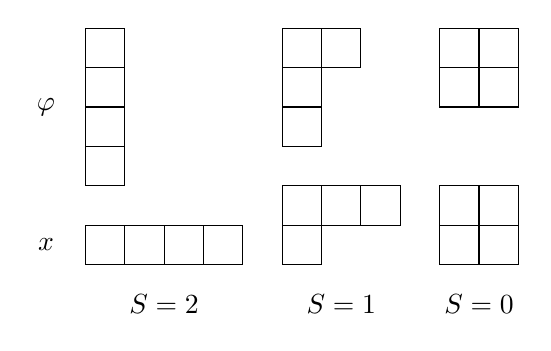
\begin{tikzpicture}
    \draw (-0.5,-1) node {$\varphi$};
    \draw (-0.5,-2.75) node {$x$};
    \draw (0,0) rectangle (0.5,-2); 
    \foreach \y in {-0.5,-1,-1.5}
    \draw (0,\y)--(0.5,\y);
    \draw (0,-2.5) rectangle (2,-3);
    \foreach \x in {0.5,1,1.5}
    \draw (\x,-2.5)--(\x,-3);
    \draw (2.5,0) rectangle (3,-1.5);
    \foreach \y in {-0.5,-1}
    \draw (2.5,\y)--(3,\y);
    \draw (3,0) rectangle (3.5,-0.5);
    \draw (2.5,-2) rectangle (4,-2.5);
    \foreach \x in {3,3.5}
    \draw (\x,-2)--(\x,-2.5);
    \draw (2.5,-2.5) rectangle (3,-3);
    \draw (4.5,0) rectangle (5.5,-1);
    \draw (5,0)--(5,-1);
    \draw (4.5,-0.5)--(5.5,-0.5);
    \draw (4.5,-2) rectangle (5.5,-3);
    \draw (5,-2)--(5,-3);
    \draw (4.5,-2.5)--(5.5,-2.5);
    \draw (1,-3.5) node {$S=2$};
    \draw (3.25,-3.5) node {$S=1$};
    \draw (5,-3.5) node {$S=0$};
  \end{tikzpicture}
  \caption{四个电子构成的杨图}
  \label{fig:4dianzi0}
\end{figure}

由图\ref{fig:4dianzi0}我们也可以明显的看出,一个杨图对应一个$S$值.如果考虑由自旋为$s$的全同粒子构成的系统,则也符合这个规则:一个杨图对就一个$S$值.粒子自旋为$s$值是,它的$z$轴分量有$2s+1$个,则杨图的行数不会超过$2s+1$.这里有一个特殊情况,如果粒子总数恰好为$2s+1$的整数倍,即$N(2s+1)$个,则杨图中有一个是每列是$2s+1$格,每行$N$格的矩形图,这图的总角动量$S$ 显然为0.同时考虑到两个角动量的合成,一个粒子角动量为$s_1$,另一个为$s_2$,则合成时的总角动量可能为:$s_1-s_2$, $s_1-s_2+1$ ,$\cdots$,$s_1+s_2$.所以只有当两个角动量值相同时,总角动量值才有可能为零,即$s_1=s_2$,时,最低总角动量值$s_1-s_2=0$.

两个多粒子系统,如果它们的总自旋为零,则表明两个系统的自旋值是相同.反应到杨图中就是两个杨图构成{\bf 互补杨图}.这里的互补,我们应当这样理解:一个杨图可以按行由多到少按左对齐排列,也可以按行由少到多右对齐排列,它们只是有一个排列形式上的不同,不会影响到对称性,所以是等价的.一个粒子系统的杨图按行由多到少左对齐排列,另一个粒子系统的杨图按行由少到多,右对齐排列,则两个杨图可以构成一个矩形.例如当$s=1$时,两个系统A和B,A由7个粒子构成,B由5个粒子构成,则考虑整体AB有12个粒子.符合粒子数是$2s+1$的倍数的关系,即
\begin{gather}
  \frac{12}{2\times 1+1}=4
\end{gather}
所以整体这个大系统$S$为零的时候构成一个$3\times4$ 的矩形杨图.如图\ref{fig:hubuyangtu}中所示,7个由实线表示的格为系统A,5个由虚线表示的格为系统B,则它们构成互补杨图,不难验证两种情况下的自旋相等关系.

\begin{figure}[H]
  \centering
  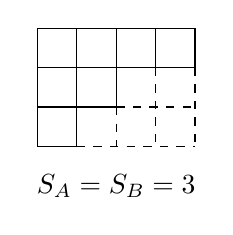
\begin{tikzpicture}
    \draw (0,0) rectangle (2,-0.5);
    \foreach \x in {0.5,1,1.5}
    \draw (\x,0)--(\x,-0.5);
    \draw (0,-0.5) rectangle (1,-1);
    \draw (0.5,-0.5)--(0.5,-1); 
    \draw (0,-1) rectangle (0.5,-1.5);
    \draw[dashed] (1,-1)--(2,-1);
    \draw[dashed] (0.5,-1.5)--(2,-1.5);
    \draw[dashed] (1,-1)--(1,-1.5);
    \draw[dashed] (1.5,-0.5)--(1.5,-1.5);
    \draw[dashed] (2,-0.5)--(2,-1.5);
    \draw (1,-2) node {$S_A=S_B=3$};
  \end{tikzpicture}
  \quad
  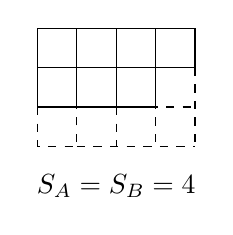
\begin{tikzpicture}
    \draw (0,0) rectangle (2,-0.5);
    \foreach \x in {0.5,1,1.5}
    \draw (\x,0)--(\x,-0.5);
    \draw (0,-0.5) rectangle (1.5,-1);
    \draw (0.5,-0.5)--(0.5,-1); 
    \draw (1,-0.5)--(1,-1); 
    \draw[dashed] (0,-1) rectangle (0.5,-1.5);
    \draw[dashed] (1,-1)--(2,-1);
    \draw[dashed] (0.5,-1.5)--(2,-1.5);
    \draw[dashed] (1,-1)--(1,-1.5);
    \draw[dashed] (1.5,-0.5)--(1.5,-1.5);
    \draw[dashed] (2,-0.5)--(2,-1.5);
    \draw (1,-2) node {$S_A=S_B=4$};
  \end{tikzpicture}
  \caption{互补杨图}
  \label{fig:hubuyangtu}
\end{figure}

下面讨论两个重要的问题.其一,自旋变量组成的杨图与自旋一般而言不是一一对应的.下面以课后题第2题来说明之.

2.系统由自旋为1的粒子组成,求种对称类型的自旋函数所具有的总自旋值$S$,设系统的粒子数为$2,3,4$.

{\bf 解:} 对双粒子系统,这个对应关系由下列事实所确立:粒子对换后,自旋波函数就乘以$(-)^{2s-S}$.对于$s=1$的粒子,由此得
\begin{figure}[H]
  \centering
  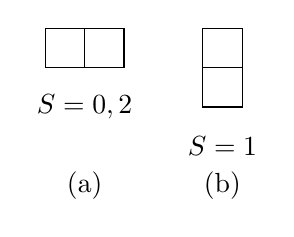
\begin{tikzpicture}
    \foreach \x in {0,0.5}
    \draw (\x,0)++(0.5,-0.5) rectangle (\x,0);
    \draw (0.5,-1) node {$S=0 , 2$};
    \draw (0.5,-2) node {(a)};
    \foreach \y in {0,-0.5}
    \draw (2,\y)++(0.5,-0.5) rectangle (2,\y);
    \draw (2.25,-1.5) node {$S=1$};
    \draw (2.25,-2) node {(b)};
  \end{tikzpicture}
  \caption{2个自旋为1的粒子}
  \label{fig:twobose}
\end{figure}
对于图\ref{fig:twobose}我们可以做如下理解:由两个粒子构成的杨图只能有这两个形式.按角动量合成规则,两个自旋为1的粒子合成,其总自旋可能值为0,1,2 .(a)波函数满足对称性,所以它只能对应$S=0$ 或者$S=2$.这里需要做出解释,为什么会有这个结果?由于自旋为1,所以杨图不会超过$2s+1=3$ 行,而这三行分别对应三个不同的$z$分量 $1$,$0$,$-1$.而这两个格只占一行,所以它可以是这三行中的任何一行,所以它所对应的$z$轴分量可以是$1+1=2$,$0+0=0$,$-1-1=-2$.总自旋为$0,1,2$ 的情况都可能出现$S_z=0$,总自旋为$2$的情况才可能有$S_z=2$,而交换对称性限定了只能$S$为偶数,所以只能是$S=0,2$.(b)满足反对称性,所以只能对应$S=1$. 这里也需要解释一下,此杨图可以对应的是三个不同$z$分量的前两行,也可心介后两行,这两种情况分别给出$S_z=1$ 和$S_z=-1$,而可以给出$S_z=\pm 1$ 的总自旋值只能是$S=1,2$,而反对称性限定了$S=1$.

对于三个粒子的情况,我们可以在2个粒子的基础上再添加一个格,具体过程参见朗道书222页,这里主要的目的是讨论结果,结果为

\begin{figure}[H]
  \centering
  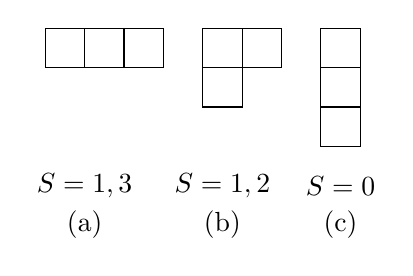
\begin{tikzpicture}
    \foreach \x in {0,0.5,1}
    \draw (\x,0)++(0.5,-0.5) rectangle (\x,0);
    \draw (0.5,-2) node {$S=1 , 3$};
    \draw (0.5,-2.5) node {(a)};
    \foreach \y in {0,-0.5}
    \draw (2,\y)++(0.5,-0.5) rectangle (2,\y);
    \draw (2.5,0)++(0.5,-0.5) rectangle (2.5,0);
    \draw (2.25,-2) node {$S=1 ,2$};
    \draw (2.25,-2.5) node {(b)};
    \foreach \y in {0,-0.5,-1}
    \draw (3.5,\y)++(0.5,-0.5) rectangle (3.5,\y);
    \draw (3.75,-2) node {$S=0$};
    \draw (3.75,-2.5) node {(c)};
  \end{tikzpicture}
  \caption{3个自旋为1的粒子}
  \label{fig:threebose}
\end{figure}

图\ref{fig:threebose} 中(a)占据一行,所以它可是占据$s_z=1,0,-1$ 的任何一行,因此总的自旋的$z$分量可能是$S_z=0,\pm 3$ ,这样的$z$分量可以由$S=0,1,2,3$产生,但是注意,这个杨图是由两个粒子的杨图\ref{fig:twobose}中的(a)演变来的,而那时的$S=0,2$,按角动量的合成,只能产生$S=1,3$ 的情况,因此图\ref{fig:threebose} 中的(a)所示的只能是$S=1,3$.还需要注意,双粒子系统,粒子交换后符号变化$(-)^{2s-S}$,但是对于三个及以上的粒子没有这个要求,所以这里的$S=1,3$ 是允许的.图\ref{fig:threebose}中(b)占据两行,可以是上两行也可以是下两行,所以它对应的总自旋$z$分量可以是$S_z=2,\pm 1$ ,产生这个分量的总自旋可以是 $S=1,2,3$,然而这个\ref{fig:threebose}中(b)也可以来源于图\ref{fig:twobose}中的(b),由角动量的合成规则,这个总自旋只能是$0,1,2$,图\ref{fig:threebose}中(b)必须同时满足这两个情况,因此其$S$值应当是按这两种情况得到的,重合的$S$值,所以其只能是$S=1,2$.图\ref{fig:threebose}中(c)只是从图\ref{fig:twobose}中(b)演变而来,其对应于$S=0,1,2$而已经判断出来\ref{fig:threebose}中(b)表示的是$S=1,2$,因此(c)必然对应$S=0$.

对于4个粒子的情况,我们可以按朗道书中的方法继续做出来,但是在这里不再继续引用.而讨论杨图所代表的$S$值时,可以按朗道书中的方法,也可以按照此处我的讨论方式.这里明确一点的是:一个杨图必定对应一个确定的$S_z$值,这个$S_z$值可以由大于等于它的不同的$S$值产生,所以一般而言,杨图与$S$值不是一一对应的.

下面再来讨论第二个问题:一个系统由自旋为$s$的粒子构成,当粒子总数为$2s+1$的整数倍时,即$N(2s+1)$个粒子,其所有的杨图中那个$(2s+1)\times N$的矩形杨图对应的总角动量为$0$.\footnote{这个问题于2019年7月14日思考一天,终于想通,记于此处.}

总自旋可以表为升降算符的形式,这个在$S_z$表像中求$\hat{S}^2$的本征值的做法一致.即
\begin{gather}
  \hat{S}^2=S_-S_++S_z^2+\hbar S_z
\end{gather}
对于这个矩形杨图显然理解为$S_z$表像中的情况,而算出$S_z=0$.同时升降算子会导致$m$值发生增减,但是每一个粒子它包含了所有$s_z$值,当$S_\pm=\sum s_\pm$作用到它上时,必然会在作用的分量上替换为其相差1的一个态,由于占据了所有的态,所以必然导致出现两个相同的态在同一列上.则

\begin{gather}
  \left<S_-S_+\right>=0
\end{gather}
于是可以判断
\begin{gather}
  \left<\hat{S}^2\right>=0
  \intertext{即}
  S(S+1)=0
\end{gather}
所以可以判断这个杨图对应的总自旋是唯一的,即$S=0$.

这个问题,也可以这样理解.杨图并没有指明表像.但是这指明了一个实际存在的状态,一个物理量的量子平均值与表像无关.这个 $(2s+1)\times N$ 的杨图,在 $S_z$  表像中理解,则显然有$S_z=0$ ,则$\left < S_z^2 \right >=0 $,同理,这个杨图也可以认为是在$S_x$表像中理解,则显然也对就$\left<S_x^2 \right>=0$,同理理解为在$S_y$表像中可得$\left<S_y^2\right>=0$,于是可以得到
$  S(S+1)=\left<S_x^2\right>+\left<S_y^2\right>+\left<S_z^2\right>=0$,
于是同样得出结论:此矩形杨图对应总自旋为0.\footnote{此处的理解是在2019年7月15日打这篇稿子时临时想到的.}

由$N(2s+1)$个自旋为$s$构成的矩形杨图对应的总自旋为0,我们可以推断出一个重要结论:自旋为$\frac{1}{2}$的粒子所构成的杨图与总自旋也一一对应.原因在于,自旋为$\frac{1}{2}$粒子所构成的杨图不会超过两行.同时一个单行的杨图必然对应一个确定的角动量,比如5个自旋为$\frac{1}{2}$的粒子构成的系统,其中排成一行的杨图如图\ref{fig:0.5fermi}所示.
\begin{figure}[H]
  \centering
  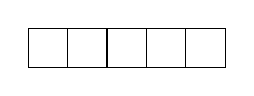
\begin{tikzpicture}
    \foreach \x in {0,0.5,1,1.5,2}
    \draw (\x,0)++(0.5,-0.5) rectangle (\x,0);
  \end{tikzpicture}
  \caption{单行1/2自旋粒子构成的系统}
  \label{fig:0.5fermi}
\end{figure}
显然此杨图所对应的总自旋$z$分量为$\frac{5}{2}$,而最大的角动量也就是$S=\frac{5}{2}$,所以此杨图对应的也只能是最大的角动量,即自旋$\frac{1}{2}$粒子构成单行杨图对应它些粒子所能构成的最大角动量,它是唯一的.

当然这5个粒子,还有其它的杨图,如图\ref{fig:0.5fermi0}所示
\begin{figure}[H]
  \centering
  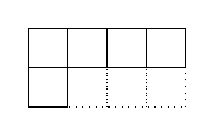
\begin{tikzpicture}
    \foreach \x in {0,0.5,1,1.5}
    \draw (\x,0)++(0.5,-0.5) rectangle (\x,0);
    \draw (0,-0.5) rectangle (0.5,-1);
    \foreach \x in {0.5,1,1.5}
    \draw [dotted] (\x,-0.5)++(0.5,-0.5) rectangle (\x,-0.5);
  \end{tikzpicture}
  \caption{两行1/2自旋粒子构成的系统}
  \label{fig:0.5fermi0}
\end{figure}
不难判断出来,互补杨图是一个单行的3格杨图,而这个单行3格杨图按前述规则,它对就一个$S'=\frac{3}{2}$的系统,而$N(2s+1)$个自旋为$s$的粒子构成的矩形杨图对应总自旋为0,按角动量的合成规则,只有两个角动量值相等的时候才会合成出总自旋为0的情况,于是互补杨图具有相同的$S$值,所以此处的5个自旋为$\frac{1}{2}$粒子所组成的系统其总自旋为$S=\frac{3}{2}$.按照这个规则一直继续下去,每一个二行杨图的互补杨图都是一个单行杨图,所以可得出结论:对于$\frac{1}{2}$粒子构成的系统,每一个杨图与总自旋是一一对应的.但是自旋不为$\frac{1}{2}$的粒子所构成的系统情况不一定成立.

\section{二次量子化---玻色统计}

设$\hat{f}^{(1)}_a$ 是粒子a的某个物理量算符,它只作用在$\xi_a$的函数上.我们可以计算出$\hat{f}^{(1)}_a$的矩阵得
\begin{gather}
  \hat{f}^{(1)}_a \psi_{p_k}(\xi_a)=\sum_l \psi_{p_l}(\xi_a)f_{lk} 
  \label{eq:twoliangzihua0}
  \intertext{上式中矩阵$f_{lk}$中省去了符号$a$,由于此矩阵与计算用的坐标无关,所以可以略去下标.即}
  f_{lk}=\int \psi_{p_l}^*(\xi) \hat{f}^{(1)}\psi_{p_k}(\xi) \mathrm{d}\xi
\end{gather}
由式\eqref{eq:twoliangzihua0}可得,当$\hat{f}^{(1)}_a$ 作用在波函$\psi_{p_k}$上时,右式可以认为是用各本征波函数展开.同时,也可以视为将波函数$\psi_{p_k}$分别取代为$\psi_{p_l}f_{lk}$,这在占有数表像中十分重要.对于由$N$个Bose 子构成的系统,波函可以写为
\begin{gather}
\left| N_1N_2\cdots \right>  
=\sqrt{\frac{N_1!N_2!\cdots}{N!}}
\sum \psi_{p_1}(\xi_1)\psi_{p_2}(\xi_2)\cdots
\end{gather}
记$\hat{F}^{(1)}$为
\begin{equation}
  \hat{F}^{(1)}=\sum_a \hat{f}^{(1)}_a
\end{equation}
将$\hat{F}^{(1)}$作用于占有数表像得
\begin{align}
  \sum_a \hat{f}^{(1)}_a \left|N_1N_2\cdots\right>&=
  \sqrt{\frac{N_1!N_2!\cdots}{N!}}
  \left\{ f_{1k}\sum \psi_{p_k}(\xi_1)\psi_{p_2}(\xi_2)\cdots\notag\right.\\
    &+f_{2k}\sum \psi_{p_1}(\xi_1)\psi_{p_k}(\xi_2)\cdots\notag\\
    &\cdots\cdots \notag\\
    &\left.+f_{Nk}\sum \psi_{p_1}(\xi_1)\psi_{p_k}(\xi_2)\cdots\psi_{p_k}(\xi_N)\right\}
\end{align}
我们考虑非零矩阵元,显然对角元不为零.下面计算之,由于在$\hat{F}^{(1)}$中对所有的坐标变量求和,则从$\psi_{p_i}$到$\psi_{p_i}$的变换一共有$N_i$项,原因在于有$N_i$个态是相同的.所以对角元为
\begin{gather}
  \left< N_i\left|\sum_a \hat{f}^{(1)}_a \right|N_i\right>=f_{ii}N_i
\end{gather}
当$\hat{F}^{(1)}$作用于某个量子态上时,相当于将此量子态消灭而重新取代了不同的态,以相同态取代的情况,上面已经求出来了.下面求出取代为不同的态的矩阵元,显然只有下列矩阵元不为零
\begin{gather}
  \left< N_i,N_k-1\left|\sum_a \hat{f}^{(1)}_a \right|N_i-1,N_k\right>=
  f_{ik} \sqrt{\frac{N_i!(N_k-1)!\cdots}{N!}}\sqrt{\frac{(N_i-1)!N_k!\cdots}{N!}}
  N_k \frac{N!}{(N_i-1)!N_k!\cdots}\notag
  \intertext{经过简单计算可得}
  \left< N_i,N_k-1\left|\sum_a \hat{f}^{(1)}_a \right|N_i-1,N_k\right>=
  f_{ik}^{(1)}\sqrt{N_iN_k}
\end{gather}

在线性谐振子中,我们遇到了升算符$\hat{a}^+$和降算符$\hat{a}$,同时有
\begin{gather}
  \left\{
    \begin{gathered}
      \hat{a}\left|n+1\right>=\sqrt{n}\left|n\right>\\
      \hat{a}^+\left|n\right>=\sqrt{n}\left|n+1\right>
    \end{gathered}
  \right.
\end{gather}
类比线性谐振子的情况,这里可以对每一个变量引入对应的升降算符
\begin{gather}
 \left\{
   \begin{gathered}
     \hat{a}_i\left|N_1,N_2,\cdots,N_i,\cdots\right>=\sqrt{N_i}\left|N_1,N_2,\cdots,N_i-1,\cdots\right>\\
     \hat{a}_i^+\left|N_1,N_2,\cdots,N_i,\cdots\right>=\sqrt{N_i+1}\left|N_1,N_2,\cdots,N_i+1,\cdots\right>
   \end{gathered}
   \right.
\end{gather}
则显然可以将$\hat{F}$表达为
\begin{equation}
  \hat{F}^{(1)}=\sum_{ik} f^{(1)}_{ik}\hat{a}_i^+\hat{a}_k
\end{equation}
这个式子之所以完全等价,原因在于据其所计算的矩阵元和直接计算的结果完全相同,但是相比直接计算,用此升降算符计算更加方便.上述结果可以方便的推广到多粒子的情况,并且计算起来可以比直接计算方便的多.比如如下替换
\begin{gather}
     \hat{F}^{(2)}=\sum_{a>b}\hat{f}^{(2)}_{ab}\notag\\
     \hat{F}^{(2)}=\frac{1}{2}\sum_{i,k,l,m}\left<ik\right|\hat{f}^{(2)}\left |lm\right>
     \hat{a}_i^+\hat{a}_k^+\hat{a}_l\hat{a}_m
\end{gather}

下面讨论整体的降算符和升算符.一个$N-1$的占有数表像可以用$N$个占有数表像,每个量子态依次减少1所形成的$N-1$个占有数的表像的线性叠加.记$N-1=N_1'+N_2'+\cdots +N_m'$,即
\begin{equation}
  \left|N_1'N_2'\cdots N_m'\right>
  =C_1\left|N_1-1,N_2,\cdots,N_m\right>
  +C_2\left|N_1,N_2-1,\cdots,N_m\right>
  +\cdots
  +C_m\left|N_1,N_2,\cdots,N_m-1\right>
  \notag
\end{equation}
在上式中各个展开系数尚未确定,这里考虑的依据是都是占有数表像,没有哪一个量子态是特殊的,所以按等概率可以考虑到每一个占有数表像出现的概率与本占有数表像的粒子数成正比.于是可得
\begin{align}
  \sqrt{N}\left|N_1'N_2'\cdots N_m'\right>
  &=\psi_1(\xi)\sqrt{N_1}\left|N_1-1,N_2,\cdots,N_m\right>\notag\\
  &+\psi_2(\xi)\sqrt{N_2}\left|N_1,N_2-1,\cdots,N_m\right>
  +\cdots
  +\psi_m(\xi)\sqrt{N_m}\left|N_1,N_2,\cdots,N_m-1\right>
  \notag
\end{align}
上式中$\psi_i(\xi)$为比例系数.于是可以引入整体降算符$\hat{\Psi}$,则
\begin{equation}
  \hat{\Psi}=\sum_{i=1}^m \psi_i(\xi)\hat{a}_i
  \label{eq:totaljiangfu}
\end{equation}
于是得
\begin{equation}
  \hat{\Psi}\left|N\right>=\sqrt{N}\left|N-1\right>
  \label{eq:totaljiangfu0}
\end{equation}
对于$\hat{\Psi}$取共轭可得$\hat{\Psi}^+=\sum_{i=1}^m \psi_i^*\hat{a}_i^+$,作用于波函数得
\begin{equation}
  \hat{\Psi}^+\left|N-1\right>=\sqrt{N}\left|N\right>
  \label{eq:totaljiangfu1}
\end{equation}
在$\hat{\Psi}$中,各$\psi_i(\xi)$为相互正交的波函数,则$\hat{F}^{(1)}$可以表达为
\begin{equation}
  \hat{F}^{(1)}=\int \hat{\Psi}^+(\xi) \hat{f}^{(1)}\hat{\Psi}(\xi)\mathrm{d}\xi
  \label{eq:totaljiangfu2}
\end{equation}

根据所引入的$\hat{\Psi}$可以得出粒子密度算符$\hat{\Psi}^+(\xi)\hat{\Psi}(\xi)$,则考虑积分
\begin{equation}
  \hat{N}=\int \hat{\Psi}^+(\xi)\hat{\Psi}(\xi)\mathrm{d}\xi=\sum_i \hat{a}^+_i\hat{a}_i
  \label{eq:totaljiangfu3}
\end{equation}
上式中$\hat{N}$即是粒子数算符.

\section{二次量子化---费米统计情形}

当有$N$个费米子时,各粒子的坐标分别以$\xi_i$来表示,其满足反对称性波函数为
\begin{equation}
  \Psi (n_1,n_2,\cdots,n_N)=\frac{1}{\sqrt{N!}}
  \begin{vmatrix}
    \Psi_{p_1}(\xi_1)&\Psi_{p_1}(\xi_2)&\cdots&\Psi_{p_1}(\xi_N)\\
    \Psi_{p_2}(\xi_1)&\Psi_{p_2}(\xi_2)&\cdots&\Psi_{p_2}(\xi_N)\\
    &&\vdots &\\
    \Psi_{p_N}(\xi_1)&\Psi_{p_N}(\xi_2)&\cdots&\Psi_{p_N}(\xi_N)
  \end{vmatrix}
\end{equation}
由于同行时行列式为零,所以不可能同一时刻有两个以上粒子处于相同的态.所以粒子的占有数要么为1要么为0,则如果超过了N个粒子,则其余的粒子占有数为0,如下表示
\footnote{此处参考了《高等量子力学》 杨泽森 著,北京大学出版社,第三版.}
\begin{equation}
  \left|N_1,N_2,\cdots\right>=\Psi(n_1,n_2)
  \qquad
  N_1=N_2=1,N_3=N_4=\cdots =0
  \label{eq:twoliangzifermi}
\end{equation}
下面直接计算$\hat{F}^{(1)}=\sum_a \hat{f}_a^{(1)}$的非零矩阵元.其中对角元显然是非零的,即
\begin{equation}
  \left<1_i\right|\hat{F}^{(1)}\left|1_i\right>=f_{ii}
  \label{eq:ercifermi0}
\end{equation}
显然上式对于$0_i$的对角元为零,所以可以写为与玻色子相同的形式为
\begin{equation}
  \left<N_i\right|\hat{F}^{(1)}\left|N_i\right>=f_{ii}N_i
  \label{eq:ercifermi1}
\end{equation}
同时,使一个占有数($N_i$)减少一个(从1变到零)另一个占有数($N_i$)增加一(从零变到1)的那些跃迁矩阵元才不等于零.当$i<k$时,显然
可得$\hat{F}^{(1)}\left|0_i,1_k\right>$ 考虑到将$\phi_{p_k}(\xi_k)$转换到$\phi_{p_i}$态组成新的行列式,然后变换行使$\phi_{p_i}$达到正常的位置(即下标按从小到大排列),这中间需要交换的行数就等于从$i+1$到$k-1$中的不为零的行数,这些不为零的行数上占有数为$1$,所以将$i+1$到$k-1$之间的所有占有数求和,则为零的那些占有数不起作用,只有占有数为$1$的那些态起作用.同时,由于一个量子态上最多有一个量子态,则不会像玻色子那样有根号项.出现的因素只能是符号项和$\hat{f}^{(1}$的矩阵元.从$i+1$ 到$k-1$ 内占有数之和记为$\sum (i+1,k-1)$,显然可得非对角非零矩阵元为
  \begin{equation}
    \left<1_i,0_k\right|\hat{F}^{(1)}\left|0_i,1_k\right>=f^{(1)}_{ik}(-)^{\sum (i+1,k-1)}
    \label{eq:ercifermi2}
  \end{equation}

  为了把算符$\hat{F}^{(1)}$也表达为类似升降算符的形式,则定义两个算符为
  \begin{equation}
    \left<0_i\right|\hat{a}_i \left|1_i\right>=\left<1_i\right|\hat{a}^+_i\left|0_i\right>=(-)^{\sum (1,i-1)}
    \label{eq:ercifermi3}
  \end{equation}
  所以两个矩阵相乘,当$i<k$时可得
  \begin{align}
    \left<1_i,0_k\right|\hat{a}_i^+\hat{a}_k\left|0_i,1_k\right>&=\left<1_i,0_k\right|\hat{a}_i^+\left|0_i,0_k\right>\left<0_i,0_k\right|\hat{a}_k\left|0_i,1_k\right>\notag\\
    &=(-)^{\sum (1,i-1)}(-)^{\sum (1,i-1)+\sum (i+1,k-1)}\notag
    \intertext{也即}
    \left<1_i,0_k\right|\hat{a}_i^+\hat{a}_k\left|0_i,1_k\right>&=(-)^{\sum (i+1,k-1)}
    \label{eq:ercifermi4}
  \end{align}
  按照$\hat{a}$在此处的定义可得
  \begin{equation}
    \hat{a}_i^+\hat{a}_i=N_i
    \label{eq:ercifermi5}
  \end{equation}
  同理交换$i,k$可得
  \begin{equation}
    \left<1_i,0_k\right|\hat{a}_k\hat{a}_i^+\left|0_i,1_k\right>=-(-)^{\sum (i+1,k-1)}
    \label{eq:ercifermi6}
  \end{equation}
  由式\eqref{eq:ercifermi6}和式\eqref{eq:ercifermi4}相加可得
  \begin{equation}
    \hat{a}_i^+\hat{a}_k+\hat{a}_k\hat{a}_i^+=0 ,\qquad i\neq k
    \label{eq:ercifermi7}
  \end{equation}
  同时可以求得
  \begin{equation}
    \hat{a}_i\hat{a}_i^+=1-N_i
    \label{eq:ercifermi8}
  \end{equation}
  同\eqref{eq:ercifermi1}对比可得
  \begin{equation}
    \hat{a}_i\hat{a}_i^++\hat{a}_i^+\hat{a}_i=1
    \label{eq:ercifermi9}
  \end{equation}
  综合式\eqref{eq:ercifermi9}和式\eqref{eq:ercifermi7}可得
  \begin{equation}
    \hat{a}_i^+\hat{a}_k+\hat{a}_k\hat{a}_i^+=\delta_{ik}
    \label{eq:ercifermi10}
  \end{equation}

